\section{Anti-derivatives}
We now want to begin to study the inverse of differentiation: the problem is, given
a function $ f $, to find some function $ F $ which has $ f $ as a derivative. Geometrically,
we are given the rate of change of a function at every point, and we wish to recover the
original function.

If $ f = F' $, then $ F $ is said to be an \emph{anti-derivative} of $ f $.

First of all, we notice that if $ F $ is an anti-derivative of $ f $ then so is $ F + C $
for any constant $ C $; this is because $ (F + C)' = F' + C' = F' + 0 = F' = f $. Thus
when we take anti-derivatives there are infinitely many different solutions that all differ
by a constant --- we cannot recover the original function given a slope function without
some more information. These functions are said to be the family of solutions that solve the
differential equation $ F' = f $; we will also write $ F(x) + C = \rint f(x) \dif{x} $ in
this case, and we say that $ F $ is the \emph{indefinite integral} of $ f $; in the
expression $ \rint f(x) \dif{x} $, $ f(x) $ is called the \emph{integrand}.

The reason for this terminology comes from the geometric meaning of the derivative --- if
$ F $ is an anti-derivative of $ f $, then $ f $ is the slope function of $ F $. This in
turn means that each value of $ f $ tells us how quickly $ F $ is rising or falling at that
point; roughly speaking, to get $ F $ back from $ f $, we need to walk along $ f $, adding
up all these infinitesimal rises and falls of $ F $ --- in other words, we need to take
all the values of $ f $, and `integrate' (combine) them together to get back the form of $ F $.

This idea is made precise in the \emph{fundamental theorem of calculus}, which we will state later on. This
same theorem tells us that if $ f $ is a continuous function then there exists some anti-derivative $ F $
of $ f $, and that this anti-derivative is unique up to a constant.

\begin{center}
  \def\arraystretch{2}
  \begin{tabular}{|c|c|c|}\hline
    \textbf{Differential equation} && \textbf{Integral equation}\\\hline
    $ f $ is the slope function of $ F $ & $\displaystyle\iff$ & $ F $ is an anti-derivative of $ f $ \\\hline
    $\displaystyle f(x) = F'(x) $ &$\displaystyle\iff$& $\displaystyle F(x) + C = \rint f(x) \dif{x} $\\\hline
    $\displaystyle f(x) = \dod{y}{x} $ &$\displaystyle\iff$& $\displaystyle y + C = \rint f(x) \dif{x} $\\\hline
  \end{tabular}
\end{center}

There are a few simple rules that we can state right away. For example, we have the following power
rule for differentiation:
\begin{displaymath}
  \od{}{x} ax^n = nax^{n - 1} \iff \rint nax^{n - 1} \dif{x} = ax^n + C
\end{displaymath}
so the anti-derivatives of $ ax^n $ are $ \frac{a}{n + 1} x^{n + 1} + C $.

Looking at the inverse power law, we notice that there is an issue when we try to anti-differentiate
$ 1/x $; the law tells us that $ \rint x^{-1} \dif{x} = \frac{1}{1 - 1} x^{0} $, which is plainly nonsense. Luckily,
last week we showed that $ \od{}{x} \ln x = 1/x $, so $ \rint 1/x \dif{x} = \ln x + C $.

Some more useful rules come by way of our differentiation arithmetic laws.
\begin{thm}
  \begin{enumerate}
    \item $ \rint 0 \dif{x} = C $ (the family of constant functions)
    \item $ \rint f(x) + g(x) \dif{x} = \rint f(x) \dif{x} + \rint g(x) \dif{x} $
    \item $ \rint \lambda f(x) \dif{x} = \lambda \rint f(x) \dif{x} $
  \end{enumerate}
\end{thm}
\begin{proof}
  \begin{enumerate}
    \item Firstly, $ \od{}{x} 0 = 0 $; so the anti-derivatives of $ 0 $ are $ 0 + C = C $.
    \item Let $ F $ and $ G $ be anti-derivatives of $ f $ and $ g $, so $ F' = f $ and $ G' = g $.
          Then $ \rint f(x) \dif{x} + \rint g(x) \dif{x} = F(x) + G(x) + C $ (*); but $ \od{}{x} [F(x) + G(x) + C] = f(x) + g(x) $
          and so $ F + G + C $ is an anti-derivative of $ f + g $ and $ \rint f(x) + g(x) \dif{x} = F(x) + G(x) + C $. Combining
          this with (*) we obtain the result.
    \item Let $ F $ be an anti-derivative of $ f $. Then $ (\lambda F)' = \lambda (F') = \lambda f $, and thus $ \lambda F $ is
          an anti-derivative of $ \lambda f $; so $ \rint \lambda f(x) \dif{x} = \lambda F(x) = \lambda \rint f(x) \dif{x} $.
  \end{enumerate}
\end{proof}

\begin{ex}
  One anti-derivative of $ y' = 3x^2 + 4 $ is $ x^3 + 4x $. Another is $ x^3 + 4x + 1 $. A third is $ x^3 + 4x + 7 $.
\end{ex}

Unfortunately, there is no `easy' way to anti-differentiate; we simply have to try to rearrange the function in some clever
way until it looks like something that we know how to deal with.

\begin{exs}\leavevmode
  \begin{enumerate}
    \item The most general antiderivative of $ \sin x $ is $ -\cos x + C $.
    \item The most general antiderivative of $ \tan x $ is $ -\ln \abs{\cos x} + C $.
    \item $ \rint \frac{1}{x + 3} \dif{x} = \ln \abs{x + 3} + C $.
    \item $ \rint \tan^2 \theta \dif{\theta} = \rint \sec^2 \theta - 1 \dif{\theta} = \tan \theta - \theta + C $.
    \item $ \rint \frac{2x}{x^2 + 1} \dif{x} = \ln \abs{x^2 + 1} + C $.
    \item $ \rint Ke^{Kx} \dif{x} = e^{Kx} + C $ for all constants $ K $.
  \end{enumerate}
\end{exs}

\begin{joke}
  Two mathematicians are in a bar. The first one says to the second that the average person knows very little about basic
  mathematics. The second one disagrees and claims that most people can cope with a reasonable amount of maths. The first
  mathematician goes off to the washroom, and in her absence the second calls over the waiter. She tells the waiter that in a few
  minutes, after her friend has returned, she will call him over and ask him a question. All he has to do is answer ``one
  third $x$ cubed.'' He repeats ``one thir-dex cue?'' She repeats ``one third $x$ cubed.'' He asks, ``one thir dex cuebd?'' ``Yes,
  that’s right,'' she says. So he agrees, and goes off mumbling to himself, ``one thir dex cuebd...''. The first mathematician returns
  and the second proposes asking the waiter for an anti-derivative to prove her point that most people do know something about basic maths;
  the first laughingly agrees. The second mathematician calls over the waiter and asks ``what is the integral of $x$ squared?'' The waiter
  says ``one third $x$ cubed'' and while walking away, turns back and says over his shoulder, ``plus a constant!''
\end{joke}

\subsection{Exercises and Problems}
\begin{enumerate}
  \item For each expression, find the most general anti-derivative with respect to $ x $.
    \begin{multicols}{2}
    \begin{enumerate}
      \item $ 2x $
      \item $ x^2 + 3x + 1 $
      \item $ \frac{1}{2\sqrt{x}} $
      \item $ x^{-3} $
      \item $ 10^x $
      \item $ \sec^2 x + \sqrt{x} $
      \item $ x\sqrt{x} $
      \item $ \sin x - \cos x $
      \item $ \frac{2x^3 + 3x - \sqrt{x}}{\sqrt[3]{x}} $
      \item $ \frac{1}{x^2} + e^x $
      \item $ \sec^2 (x + 1) $
    \end{enumerate}
    \end{multicols}
  \item Verify the examples in the notes by differentiation.
  \item Show that $ \rint 3x^2 + 4x + 5 + \frac{2}{x} \dif{x} = x^3 + 2x^2 + 5x + \ln x^2 + C $.
  \item If $ \od{y}{t} = 1.5 \sqrt{t} $ and $ y(4) = 10 $, find $ y(t) $ exactly.
  \item Find $ f $ if $ f''(x) = 12x^2 + 6x - 4 $, $ f(0) = 4 $, $ f(1) = 1 $.
  \item The velocity of a particle is given by $ v(t) = 2t + 1 $. Find its position at $ t = 4 $
        if its position at $ t = 0 $ is $ x = 0 $.
  \item The acceleration of a particle is given by $ a(t) = 10\sin t + 3\cos t $. At $ t = 0 $, its position is $ x = 0 $; at $ t = 2\pi $,
        its position is $ x = 12 $. Find its position at $ t = \frac{\pi}{2} $.
  \item Starting from rest, a car takes $ T $ seconds to reach its maximum speed, $ v_\text{max} $. A plausible
        model for the velocity of the car after $ t $ seconds is
        \begin{displaymath}
          v(t) = \begin{cases} v_\text{max} \left( \frac{2t}{T} - \frac{t^2}{T^2} \right) & t \leq T, \\ v_\text{max} & t \geq T. \end{cases}
        \end{displaymath}
    \begin{enumerate}
      \item Write an expression for $ a_\text{max} $, the maximum acceleration attained by the car.
      \item Show that the distance travelled by the car from the time it starts to the point it reaches its maximum
            speed is given by $ s(t) = \frac{1}{3} a_\text{max} T^2 $.
    \end{enumerate}
  \item Find all functions $ g $ such that $ g'(x) = 4 \sin x + \frac{2x^5 - \sqrt{x}}{x} $.
  \item For each function, sketch an anti-derivative passing through $ (0, 0) $:
        \begin{center}
          \begin{tabular}{ccc}
            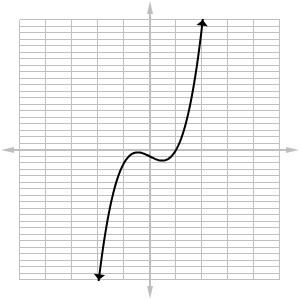
\includegraphics[width=0.28\textwidth]{anti1}&
            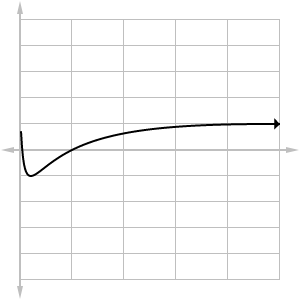
\includegraphics[width=0.28\textwidth]{anti2}&
            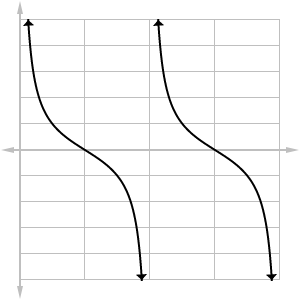
\includegraphics[width=0.28\textwidth]{anti3}\\
            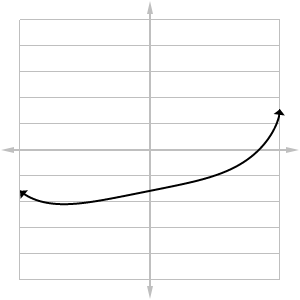
\includegraphics[width=0.28\textwidth]{anti4}&
            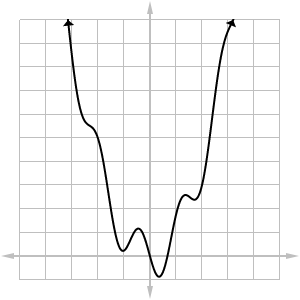
\includegraphics[width=0.28\textwidth]{anti5}&
            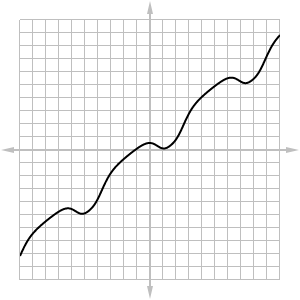
\includegraphics[width=0.28\textwidth]{anti6}
          \end{tabular}
        \end{center}
  \item Show that if $ F $ is an anti-derivative of $ f $, $ G $ is an anti-derivative of $ g $, and $ \alpha $ and $ \beta $ are any constants,
        then $ \alpha F + \beta G $ is an anti-derivative of $ \alpha f + \beta g $.
  \item Give an example of functions $ f $ and $ g $ such that if $ F $ and $ G $ are anti-derivatives of $ f $ and $ g $ respectively then $ FG $
        is \emph{not} an anti-derivative of $ fg $.
\end{enumerate}

\subsection{References}
Because of the way we're covering integration, most books will have problems which we can't
do yet (for example, $ \rint 1/x \dif{x} $). That said, many more anti-differentiation problems
can be found in the following: Stewart, section 4.4; Thompson, chapter XVIII.

\subsection{Homework}
\paragraph{Reading}
In mathematics there are a lot of examples of operations which are easy to perform
in one direction, but harder to reverse.

\begin{center}
  \begin{tabular}{c|c}
    \textbf{Easy} & \textbf{Hard}\\
    addition & subtraction\\
    multiplication & division\\
    expanding & factorising\\
    exponents & logarithms\\
    tying a knot & unravelling a knot\\
    differentiation & anti-differentiation
  \end{tabular}
\end{center}

One very important application of this idea is in cryptography. Most modern computer
systems are dependent on something known as the RSA cipher, which essentially relies
on the fact that it's much easier to multiply large primes together than it is to
work out what primes divide a large integer.

Anti-differentiation in particular is very difficult, in the sense that there are
rules that enable us to take the derivative of every combination of `simple' functions
(polynomials, exponentials, logarithms, trig functions, sums, products, functions of
functions) --- but there are some functions, made up of these building blocks, which
do not have anti-derivatives of the same type.

For example, there is no anti-derivative of $ x^x $ which can be produced with simple
functions. There is a function $ f $ such that $ f'(x) = x^x $, we just can't write it
down at all using any combination of these building blocks despite the function $ x \mapsto x^x $
being made up of them.

\paragraph{Problems}
\begin{enumerate}
  \item Find the most general anti-derivative.
    \begin{enumerate}
      \item $ f(x) = x - 3 $
      \item $ f(x) = (x + 1)(x + 2) $
      \item $ f(\theta) = 6\theta^2 - 7 \sec^2 \theta $
      \item $ g(h) = \pi^2 $
      \item $ f(x) = x^{3.7} + \sqrt{x} + 7x^{\sqrt{7} - 1} $
    \end{enumerate}
  \item Given that the graph of $ \varphi $ passes through the point $ (1, 6) $
        and that the slope of its tangent line at $ (x, \varphi(x)) $ is $ 2x + 1 $,
        find $ \varphi(2) $.
  \item This is the second derivative of $ g $. Find $ g $ given that $ g'(0) = 0 $ and $ g(0) = 1 $.
        \begin{center}
          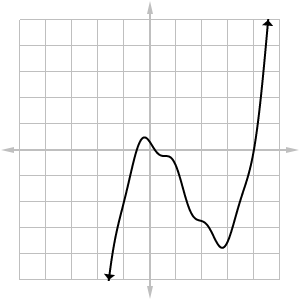
\includegraphics[width=0.4\textwidth]{anti7}
        \end{center}
\end{enumerate}
